%\begin{tcolorbox}[title=TODO]
%Measurement results / analysis / discussion: 1/3
%\begin{itemize}
%\item whatever you have done, you must comment it, compare it to other systems, evaluate it
%\item usually, adequate graphs help to show the benefits of your approach
%\item caution: each result/graph must be discussed! what's the reason for this peak or why have you ovserved this effect
%\end{itemize}
%\end{tcolorbox}

\section{Image Size}
We were able to create a minimal \ac{OS} image with the Azure IoT Edge runtime
using \textit{reUpNix}. To achieve this, we created \textit{Nix} derivations
and modules for the \textit{Azure IoT Edge} runtime and the \textit{Azure IoT Edge
Identity Service}. We also created a \textit{Nix} derivation for the \ac{ADU} Agent.
Microsoft has the source code for the previously mentioned components
publicly available on GitHub, so we could build the \textit{Nix} packages directly
from source, which is written in Rust and C and uses Cargo and CMake respectively.
Further, we had to add the already existing \textit{Nix} package for \textit{Docker}
to the system configuration. Finally, since \textit{reUpNix} removes some unnecessary
Kernel modules, we had to add Kernel modules back to the system configuration in order
to be able to run \textit{Docker}. Most notably, we had to add the modules
\textit{br\_netfilter}, \textit{xt\_nat} and \textit{8021q} to the system configuration,
since they are required for \textit{Docker} networking.

We compared \textit{reUpNix}, \textit{NixOS 23.01}, \textit{Ubuntu 22.04}, and
\textit{Yocto Kirkstone} by their installed image size, with the methodology introduced
in chapter \ref{sec:image-size}. All system images feature an \ac{OCI}-compliant container runtime
and the Azure IoT Edge runtime. The results of the comparison are shown in table \ref{tab:image-size}.

\begin{table}[H]
	\centering
	\begin{tabular}{l|l|l}
	\toprule
		Operating System & Image Variation 1 & $\Delta$ Ubuntu\\
	\midrule
    \textbf{reUpNix} & \text{1 289 MB} & \color{ba-green}{- 1 010 MB} \\
    \textbf{NixOS 23.01} & \text{2 361 MB} & \textcolor{ba-red}{+ 62 MB} \\
    \textbf{Ubuntu 22.04} & \text{2 299 MB} & \text{-} \\
    \textbf{Yocto Kirkstone} & \text{4 933 MB} & \textcolor{ba-red}{+ 2 634 MB} \\
	\bottomrule
	\end{tabular}
	\caption{Image size by OS for each variation}
	\label{tab:image-size}
\end{table}
\noindent
We can see from table \ref{tab:image-size} that with its 1,289 Megabytes
\textit{reUpNix} has a 43\% smaller base image size than Microsoft's recommended
\textit{Ubuntu 22.04}. It is also 45\% smaller than the base image size of
\textit{NixOS 23.01}, which shows that the minification process is very effective
in minimizing the size of the \ac{OS} on disk despite having a fully working
Azure IoT Edge runtime installed.
To further illustrate the differences in size, refer to figure \ref{fig:image-size}.


\begin{figure}[htbp]
  \centering
  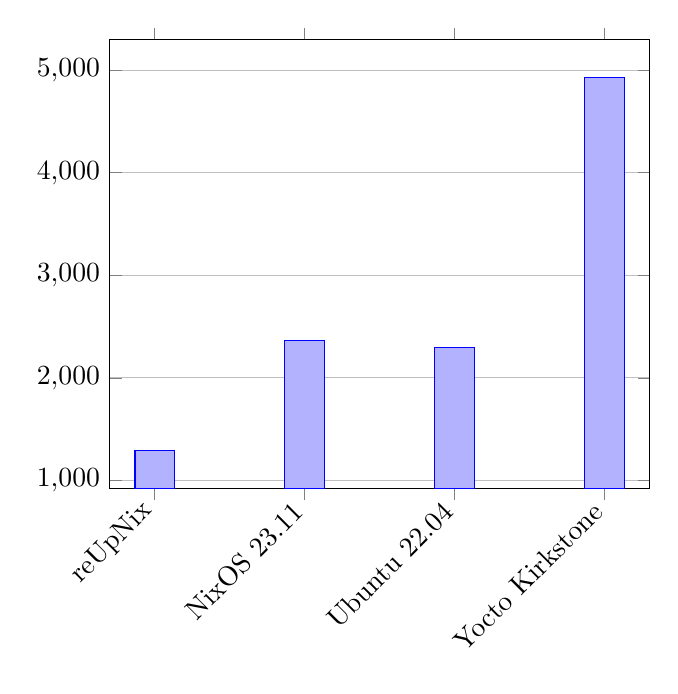
\begin{tikzpicture}
    \begin{axis}[
      ybar,
      bar width=0.5cm,
      % width=0.5\textwidth,
      % height=0.5\textwidth,
      xtick=data,
      xticklabels={
        {reUpNix},
        {NixOS 23.11},
        {Ubuntu 22.04},
        {Yocto Kirkstone}
      },
      x tick label style={rotate=45,anchor=east}, % Rotating labels
      ymajorgrids=true, % Major grid lines for y-axis
      ytick={0,1000,2000,3000,4000,5000}, % Y-axis tick marks
      extra y ticks={1000,2000,3000,4000}, % Additional y-axis tick marks
      extra y tick labels={}, % Remove labels for the extra ticks
      ]

      \addplot coordinates {
        (1,1289)
        (2,2361)
        (3,2299)
        (4,4933)
      };

    \end{axis}
  \end{tikzpicture}
\caption{Image size by OS in Megabytes}
\label{fig:image-size}
\end{figure}

\noindent
In contrary, the difference in image size between \textit{Ubuntu 22.04} and
\textit{NixOS} is only 62 Megabytes, which is unsurprising, since both are
general purpose \textit{Linux} distributions and not specifically designed
for embedded and \ac{IoT} systems. The largest image in this comparison is
\textit{Yocto Kirkstone}, which is 2,634 Megabytes larger than \textit{Ubuntu 22.04}.
However, it features no effort to minimize the size of the \ac{OS} and it
just contains a default development configuration of the \textit{Yocto Project}
for \textit{Azure IoT Edge}.

\clearpage

\section{Update size}
\begin{table}[H]
	\centering
	\begin{tabular}{l|l|l}
	\toprule
		Operating System & Image Variation 1 & $\Delta$ Ubuntu\\
	\midrule
    \textbf{reUpNix} & \text{1 289 MB} & \color{ba-green}{- 1 010 MB} \\
    \textbf{NixOS 23.01} & \text{2 361 MB} & \textcolor{ba-red}{+ 62 MB} \\
    \textbf{Ubuntu 22.04} & \text{2 299 MB} & \text{-} \\
    \textbf{Yocto Kirkstone} & \text{4 933 MB} & \textcolor{ba-red}{+ 2 634 MB} \\
	\bottomrule
	\end{tabular}
	\caption{Update size by OS for each variation}
\end{table}

\begin{figure}[htbp]
  \centering
  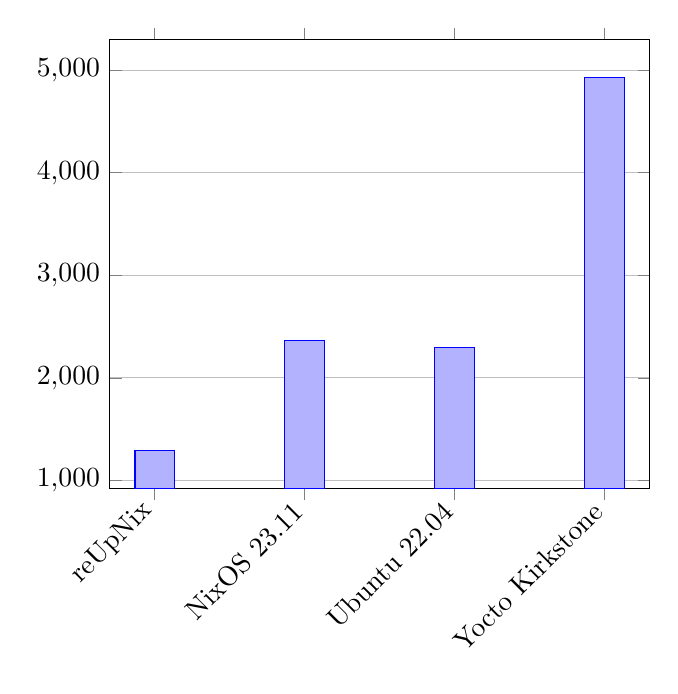
\begin{tikzpicture}
    \begin{axis}[
      ybar,
      bar width=0.5cm,
      % width=0.5\textwidth,
      % height=0.5\textwidth,
      xtick=data,
      xticklabels={
        {reUpNix},
        {NixOS 23.11},
        {Ubuntu 22.04},
        {Yocto Kirkstone}
      },
      x tick label style={rotate=45,anchor=east}, % Rotating labels
      ymajorgrids=true, % Major grid lines for y-axis
      ytick={0,1000,2000,3000,4000,5000}, % Y-axis tick marks
      extra y ticks={1000,2000,3000,4000}, % Additional y-axis tick marks
      extra y tick labels={}, % Remove labels for the extra ticks
      ]

      \addplot coordinates {
        (1,1289)
        (2,2361)
        (3,2299)
        (4,4933)
      };

    \end{axis}
  \end{tikzpicture}
\caption{Update Size by OS in Megabytes}
\end{figure}

\clearpage

\section{Time To Recover}
\begin{lstlisting}[
    caption={Sample App Which Sends The Current Timestamp Startup},
    label=lst:sampleapp]
namespace BA.SampleApp;

using System.Encoding;
using Microsoft.Azure.Devices.Client;

public class Program
{
  public static async Task Main(string[] args)
  {
    var currentTime = DateTime.UtcNow.ToString();
    var client = new DeviceClient.CreateFromEnvironment();
    var messageBytes = Encoding.UTF8.GetBytes(currentTime);
    var message = new Message(messageBytes);

    await client.SendEventAsync(message);
  }
}
\end{lstlisting}

\begin{table}[H]
	\centering
	\begin{tabular}{l|l|l|l}
	\toprule
		Operating System & Mean & Std. Deviation & Std. Error \\
	\midrule
    \textbf{reUpNix} & 1.0 & 1.0 & 1.0 \\
    \textbf{NixOS 23.01} & 1.0 & 1.0 & 1.0 \\
    \textbf{Ubuntu 22.04} & 1.0 & 1.0 & 1.0 \\
    \textbf{Yocto Kirkstone} & 1.0 & 1.0 & 1.0 \\
	\bottomrule
	\end{tabular}
	\caption{Time to recover by OS in seconds}
	\label{tab:timetorecover}
\end{table}

\begin{figure}[H]
\centering
\begin{tikzpicture}
  \begin{axis}[
    title  = ReUpNix,
    ybar,
    enlarge y limits  = {0.15,upper},
    width = 0.5\textwidth,
    nodes near coords,
  ]
    \addplot table [x=seconds, y=times, col sep=comma] {data/time-to-recover-reupnix.csv};
  \end{axis}
\end{tikzpicture}
\begin{tikzpicture}
  \begin{axis}[
    title  = NixOS,
    ybar,
    enlarge y limits  = {0.15,upper},
    width = 0.5\textwidth,
    nodes near coords,
  ]
    \addplot table [x=seconds, y=times, col sep=comma] {data/time-to-recover-nixos.csv};
  \end{axis}
\end{tikzpicture}
\begin{tikzpicture}
  \begin{axis}[
    title  = Ubuntu 22.04,
    ybar,
    enlarge y limits  = {0.15,upper},
    width = 0.5\textwidth,
    nodes near coords,
  ]
    \addplot table [x=seconds, y=times, col sep=comma] {data/time-to-recover-ubuntu.csv};
  \end{axis}
\end{tikzpicture}
\begin{tikzpicture}
  \begin{axis}[
    title  = Yocto Kirkstone,
    ybar,
    enlarge y limits  = {0.15,upper},
    width = 0.5\textwidth,
    nodes near coords,
  ]
    \addplot table [x=seconds, y=times, col sep=comma] {data/time-to-recover-yocto.csv};
  \end{axis}
\end{tikzpicture}
\caption{Time of recovery after a reboot by OS in seconds.}
\end{figure}

\clearpage
\section{Container Updates}


\begin{figure}[htbp]
  \centering
  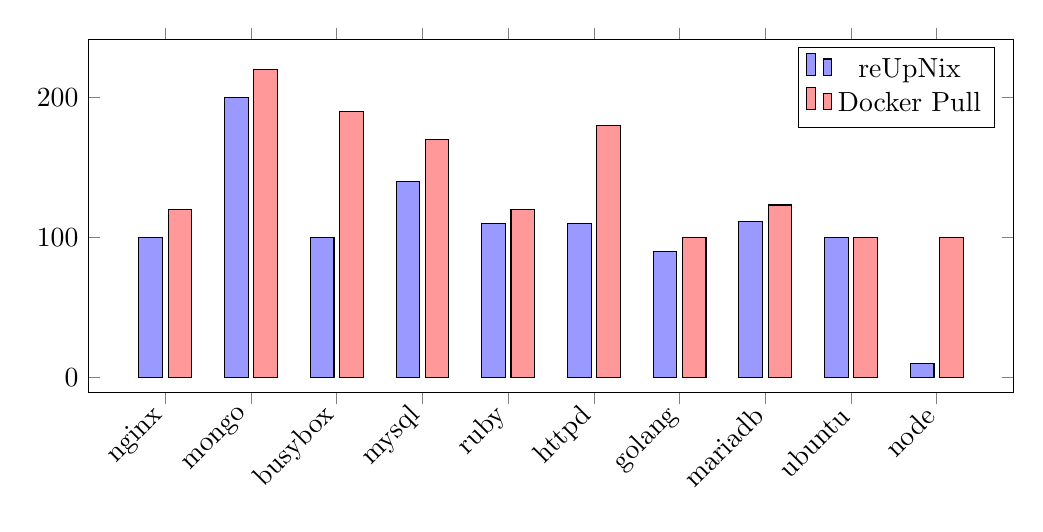
\begin{tikzpicture}
    \begin{axis}[
      ybar,
      bar width=0.5cm,
      width=1.1\textwidth,
      height=0.5\textwidth,
      bar width=0.3cm, % Decrease the bar width
      % xlabel={Container Image},
      % ylabel={Download Size},
      xtick=data,
      xticklabels={
        nginx, mongo, busybox, mysql, ruby, httpd, golang, mariadb, ubuntu, node
      },
      x tick label style={rotate=45,anchor=east},
      ]

      \addplot[fill=blue!40] coordinates {
        (1,100) % nginx
        (2,200) % mongo
        (3,100) % busybox
        (4,140) % mysql
        (5,110) % ruby
        (6,110) % httpd
        (7,90)  % golang
        (8,111) % mariadb
        (9,100) % ubuntu
        (10,10) % node
      };

      \addplot[fill=red!40] coordinates {
        (1,120) % nginx
        (2,220) % mongo
        (3,190) % busybox
        (4,170) % mysql
        (5,120) % ruby
        (6,180) % httpd
        (7,100) % golang
        (8,123) % mariadb
        (9,100) % ubuntu
        (10,100) % node
      };

      \legend{reUpNix, Docker Pull}
    \end{axis}
  \end{tikzpicture}
  \caption{Container Image Download Size}
  \label{fig:container_download_size}
\end{figure}
